\documentclass{article}
\usepackage{graphicx}
\usepackage{amssymb}
\usepackage{amsthm}
\usepackage{hyperref}
\usepackage{kotex}
\title{Delaunay Triangulation Algorithm}
\begin{document}
\maketitle
\begin{abstract}
    이 저작물은 베를린 자유대학 Faniry H. Razafindrazaka 박사의 아래 논문을
    들로네 삼각분할에 대해서만 번역한 것입니다.번역자 정요한. 
    \url{http://page.mi.fu-berlin.de/FANIRY/files/faniry_aims.pdf}
\end{abstract}
\section{introduction}
점들로 이루어진 집합에 대해 들로네 삼각분할을 수행 하는 것은 계산 기하학의 1
고전적인 문제다. 이 문제는 1934년에 프랑스인 수학자 Boris Nikolaevich Delone(Delaunay)가
1934년 발견하였다. 이 문제에 대해서 수학자와 컴퓨터 과학자들이 많은 
알고리즘들을 제시하고 있다. 그 중, 1985년에 Guibas 와 Stolfi가 제안한 
분할정복 기법을 이용하여 $O ( n \log n)$에 수행 가능 하다. 
그리고 조금 후, Steve Fortune은 이와 같은 복잡도를 가지는 Sweepline 알고리즘을 
제시했다. 이 알고리즘은 voronoi diagram을 위해 작성된 것이다. 
그런데 이 알고리즘은 구현하기 힘들기에 엔지니어들은 이것보다는 
incremental insertion 알고리즘을 사용한다. 이 알고리즘은  
단순명료하고 구현이 그렇게 어렵지 않다. Guibas와 Stolfi가 제시한 
incremental insertion은 점을 찾는데 걷기 전략walking strategy를 이용하는데 
그 복잡도가 $O(n^{1/2})$이다. Mucke는 이 알고리즘을 개선하여 $O(n^{1/3})$
복잡도를 달성하였다. 이 알고리즘들은 좋은 구현법이지만, 최적 알고리즘은 아니다. 
우리는 점을 찾는데에 DAG(Directed Acyclic Graph)-based 자료구조를 사용한 
최적 랜덤화 incremental algorithm을 사용할 것이다. 이 알고리즘은 평균 시간복잡도 
$O(n \log n)$ 이며, 공간복잡도 $O(n)$을 소요한다. 

(generating artificial terrains with delaunay triangulation 은 번역을 제외한다.)

이 작업은 두 부분으로 나뉜다. 첫 번째 파트는 들로네 삼각분할과 알고리즘의 
이론적인 분석이고, 두 번째 파트는 지역 생성과 관련한 알고리즘의 응용이다. 
들로네 삼각분할은 보로노이 다이어그램과 쌍대dual로 알려져있다. 챕터 2에서 
이에 대해 이야기할 것이며, 들로네 삼각형의 특성인 empty circle 특징 부터 
지역적 최대-최소 각도 특징까지 학습할 것이다. 챕터 3에서는 몇 알고리즘들이 
주어질것이며, 랜덤화 incremetal method와 비교해볼 것이다. 특히 분할정복 기법과
plane sweep 알고리즘이 될 것 이다. 챕터 4에서는 DAG-based 자료구조를 이용한 
알고리즘을 이야기 할 것이다. 알고리즘의 모든 부분의 스도코드가 제공 될 것이며, 
확률론과 backwards analysis에서 사용되는 기본적인 도구를 이용하여 - 최대한 
간략하게 알고리즘에 대한 분석을 수행하고자 한다. 
\pagebreak
\section{보로노이 다이어그램과 들로네 삼각분할}
이 섹션에서는 voronoi cells, half-planes의 정의를 알아볼 것이다. 
그리고 나서 들로네 삼각분할의 쌍대 특징에 대해 이야기 해 볼 것이다. 
\subsection{보로노이 다이어그램}  
\subsubsection{보로노이 셀}
$\mathcal{P} = \{ p_1, p_2, p_3, ... , p_n \} $을 유클리디안 평면에 존재하는 
구역안에 있는 점의 집합이라 하자. 이 평면 위에 존재하는 구역을 보로노이 셀이라고 하며 
다음 조건을 만족한다. 구역 $p_i$에 가까이 존재하는 모든 점들은 보로노이 셀 
$\mathcal{V}(p_i)$라 한다. 
\[
    \mathcal{V}(p_i) = \{x \in \mathbb{R}^2:d(x, p_i) \le d(x, p_j), \forall i \ne j \}
\]
즉, 다른 점들보다 점 $p_i$와 가까운 공간을 대해 $\mathcal{V}(p_i)$라고 한다. 
공간상의 어떤 지점들은 하나 이상의 점들과 같은 거리를 가지고 있다. 이 지점들의 집합을 
voronoi diagram 이라고 한다. $\mathcal{V}(\mathcal{P})$. 

\subsubsection{Example}

평면 위의 세 구역을 고려해보자. 기하학적으로, 보로노이 다이어그램은 세 지점이 이루는 
삼각형을 수직이등분하게된다. 이 세 선은 이 삼각형의 외접원의 중심에서 교차하게 된다. 

\begin{figure}[h]
    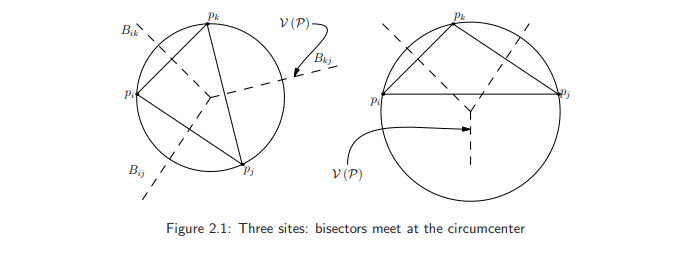
\includegraphics{capture.PNG}
\end{figure}

\subsubsection{Half-Planes}

$H(p_i, p_j)$를 $B_{ij}$에 의해 나누어지고 $p_i$를 포함하는 반평면이라고 한다. $H(p_i,p_j)$를 
다음과 같이 정의할 수 있다. 
$$
H(p_i, p_j) = \{ x \in \mathbb{R}^2 | d(x, p_i) < d(x, p_j) \}, i \ne j,
$$ 
이 표기를 이용하여 보로노이 다이어그램을 다음과 같이 정의 할 수 있다. 
$$
\mathcal{V}(p_i) = \bigcap_{j \ne i}H(p_i, p_j), \forall j.
$$
교집합은 $i$와 다른 모든 $j$에 대해 수행한다. 

\subsection{Dual of $\mathcal{V}(\mathcal{P})$}

\textbf{definition 2.2.1} 평면 그래프 G에 대한 쌍대는 다음과 같이 생성될 수 있다. 
G의 각 면은 vertex로 표현되고, 그 vertex 간에 간선을 그리면 
간선 $e \in E(G)$은 기존 그래프에서 경계를 맞대고 있는 면들을 표현한다.  

\textbf{definition 2.2.2} 점 집합 $\mathcal{P}$의 삼각분할은 부분 평면 S.... 문소리고 해석안됨 

\subsubsection {Construction}

1934년, 들로네는 보로노이 다이어그램의 쌍대 그래프가 보로노이 셀 $\mathcal{P}$  
을 삼각분할 한다는 것을 증명했다. 보로노이 셀을 삼각분할 한 것을 들로네 삼각분할 
$\mathcal{D}()\mathcal{P}$라 한다. 아래 그림은 보로노이 다이어그램 $n=11$ 셀과 
그에 대응하는 쌍대 그래프, 들로네 삼각분할이다. 

\begin{figure}[h]
    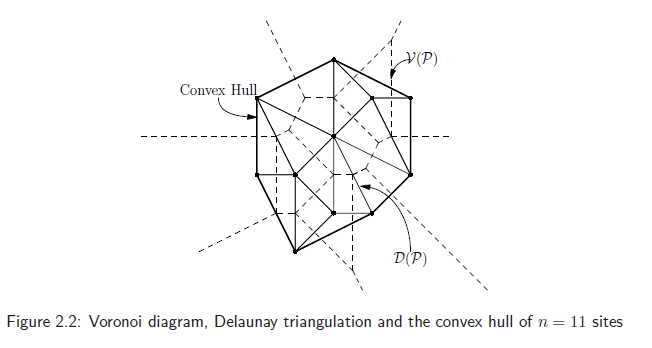
\includegraphics{capture2.PNG}
\end{figure}

\subsubsection{Duality Properties} 

이 보로노이 다이어그램 그래프의 쌍대 그래프는 edges, vertices, faces에 대해 
일대일 대응하는 성격을 띈다. 아래는 그 관찰에 대해 정리한 것이다. 

\textbf{D1.} $\mathcal{D}(\mathcal{P})$는 $\mathcal{V}(\mathcal{P})$의 
쌍대 그래프이다. 

\textbf{D2.} 네 점 $\mathcal{P}$가 같은 외접원 안에 포함되지 않는다면, 
$\mathcal{D}(\mathcal{P})$는 삼각분할이다. (see 2.3.2)

\textbf{D3.}  $\mathcal{D}(\mathcal{P})$의 모든 삼각형은 
$\mathcal{V}(\mathcal{P})$의 vertex와 대응한다. 

\textbf{D4.}  $\mathcal{D}(\mathcal{P})$의 모든 edge은 
$\mathcal{V}(\mathcal{P})$의 edge와 1:1 대응한다. 

\textbf{D5.}  $\mathcal{D}(\mathcal{P})$의 모든 vertex는 
$\mathcal{V}(\mathcal{P})$의 faces(cell)와 1:1 대응한다. 

\textbf{D6.}  $\mathcal{D}(\mathcal{P})$의 외곽 경계는 
$\mathcal{P}$의 convex hull 이다. 

\textbf{D7.}  $\mathcal{D}(\mathcal{P})$의 열등 삼각형들은 
vertex를 포함하지 않는다. 

\textbf{Remark 2.2.3} 

\subsection{The Delaunay triangulation}
    
\section{The Algorithm}





\end{document}